\section{Sprint 6}
\subsection{Sprint summary}
Sprint 6 was aimed at completing all functionality with the application to allow for user testing and rigorous testing and bug fixing. Completing the persistence layer was crucial to testing all the applications functionality. All tabs were to be completed at the end of this sprint. The only exception would be particularly tricky problems that required more resources that what were initially allocated.

\subsection{Sprint burndown}



\begin{figure}[H]
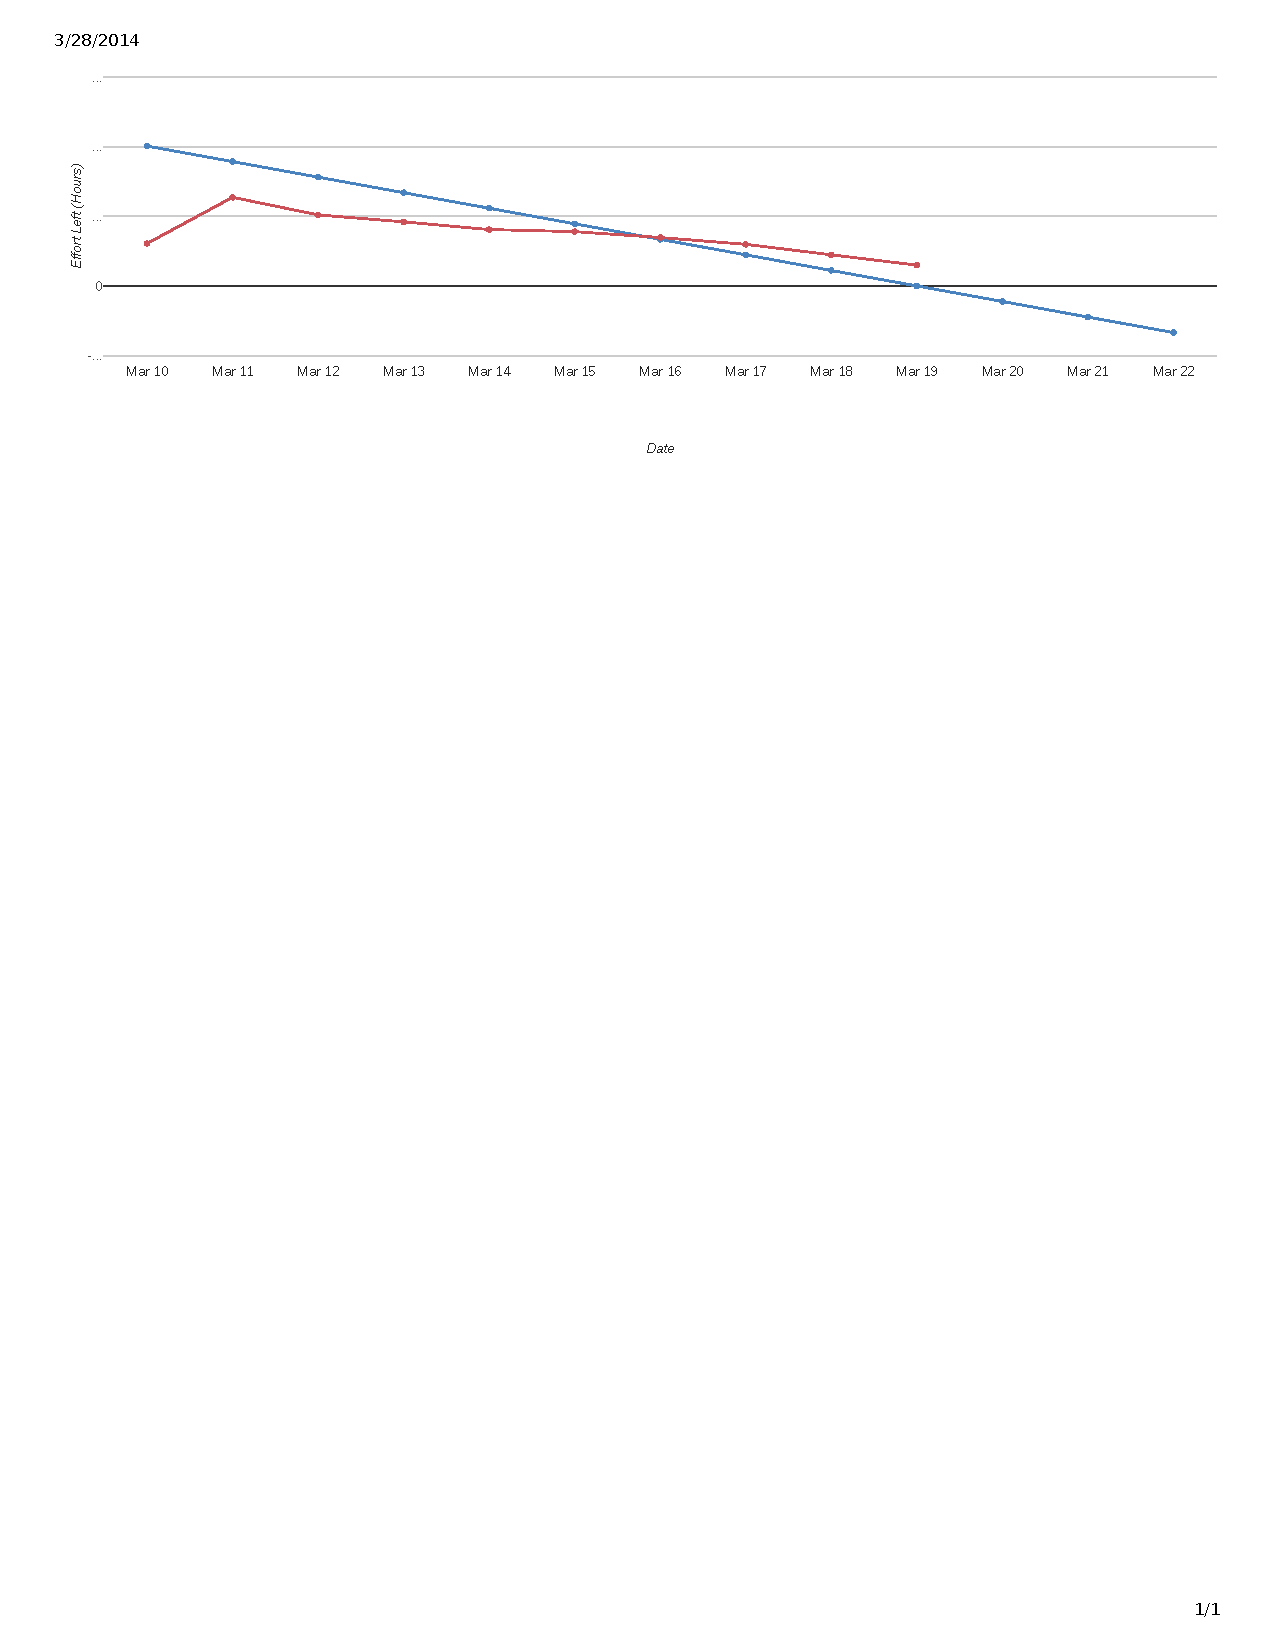
\includegraphics[width=\textwidth, trim= 1cm 21cm 1cm 1cm, clip=true]{ch/projectManagement/fig/burndown4.pdf}
\caption{Sprint 6 burndown chart}
\label{fig:sprint6burndown}
\end{figure}

\subsection{Sprint backlog}

The backlog and time usage result.

\begin{table}[H]
	\begin{tabular}{|l|p{7cm}|p{2.2cm}|p{1.5cm}|p{1.5cm}|}%
		\hline \bfseries User story & \bfseries Details & \bfseries Hours\newline estimated & \bfseries Hours spent & \bfseries Hours left
		\csvreader[head to column names]{ch/projectManagement/sec/sprints/sprint6/userstories.csv}{}% use head of csv as column names
		{\\\hline \id & \title & \estimated & \spent & \left} \\\hline% specify your coloumns here
	\end{tabular}
    \caption{Sprint 3 backlog}
\end{table}
\subsection{Issues and solutions}
One of the prevalent issues through the entire project was the fact that many of the team members had no prior knowledge to Android or its development environment. This lead to a steep learning curve for the members in question. This also became a problem in sprint 6 

\subsection{Work done}
Server and client implementations for the data sync were finished relatively early in the sprint. This allowed all data stored locally to be synchronized with the servers representation of the user. All the tabs with Facebook integration were also mostly finished. Users tests were also conducted to allow for last minute adjustments on the GUI if that was found to be necessary. 

\subsection{Sprint review}
After looking at the progress of sprint 6, the team decided it was time to dedicate some resources to the report in order to not fall behind. Sprint 5 and 6 had been devoted almost exclusively to development in order to meet deadlines set in cooperation with the customer. Even though generous estimates were made to ensure delivery, the team divided into two groups as an extra precaution. 